\chapter{Methodology}
\label{chap:methodology}



\section{System Design}
\label{sec:system-design}

Our neuro-symbolic planning system extends a re-implementation of the Generative Agents architecture \cite{parkGenerativeAgentsInteractive2023a} with modifications enabling a controlled comparison between purely neural planning (baseline) and neuro-symbolic planning (our approach).

\subsection{System Architecture}
\label{subsec:system-architecture}

The implementation transforms the original monolithic Generative Agents codebase into a modular, service-oriented architecture:

\begin{enumerate}
  \item \textbf{Repository Layer}: Abstracts external dependencies (LLM APIs, file storage) behind interfaces. \texttt{LLMRepository} supports both OpenAI (production) and mock providers (testing). \texttt{EnvironmentRepository} abstracts world state persistence.

  \item \textbf{Service Layer}: Encapsulates cognitive capabilities in swappable interfaces:
        \begin{itemize}
          \item \texttt{PlanningService}: Daily planning and task decomposition
          \item \texttt{DialogueService}: Conversation generation
          \item \texttt{PerceptionService}: Environment observation and memory retrieval
          \item \texttt{ReflectionService}: Memory summarization
          \item \texttt{EnvironmentService}: Spatial navigation and object interaction
        \end{itemize}

  \item \textbf{Orchestration Layer}: The simulation loop consumes services through interfaces, configured via environment variables (\texttt{LLM\_PROVIDER}, \texttt{PLAN\_MODULE}) controlling which implementations run.
\end{enumerate}

\textbf{Key Design Principle}: The \texttt{PlanningService} abstraction enables side-by-side comparison of baseline (LLM-only hierarchical planning) and neuro-symbolic planning by ensuring both share identical environment state, memory retrieval, and LLM infrastructure. Only the planning logic differs, isolating the independent variable.

\begin{figure}[H]
  \centering
  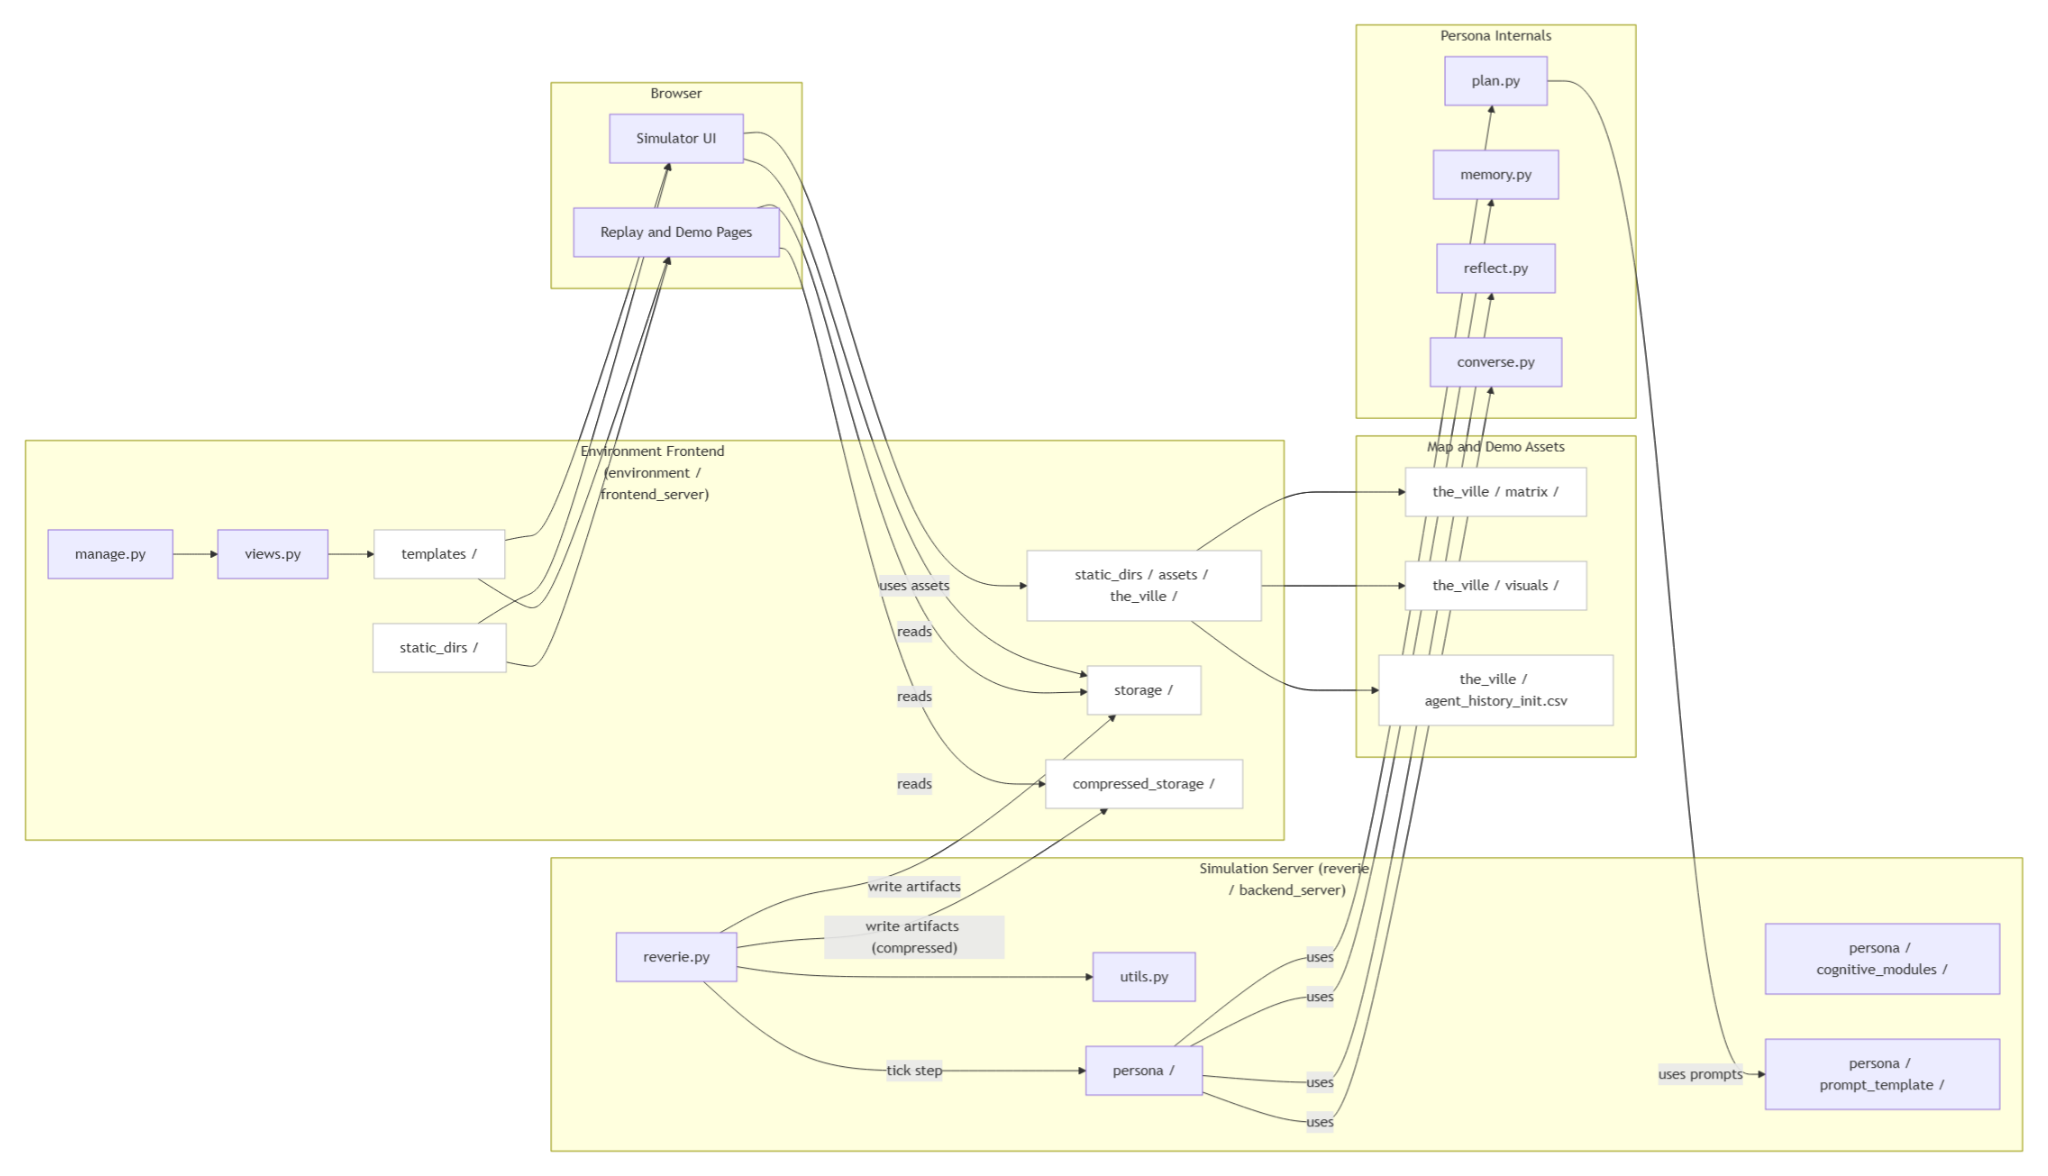
\includegraphics[width=\textwidth]{Pictures/Code Structure - before.png}
  \caption{Original monolithic architecture from the Generative Agents codebase \cite{parkGenerativeAgentsInteractive2023a}, showing tightly coupled components without clear separation of concerns.}
  \label{fig:code-structure-architecture-before}
\end{figure}

\begin{figure}[H]
  \centering
  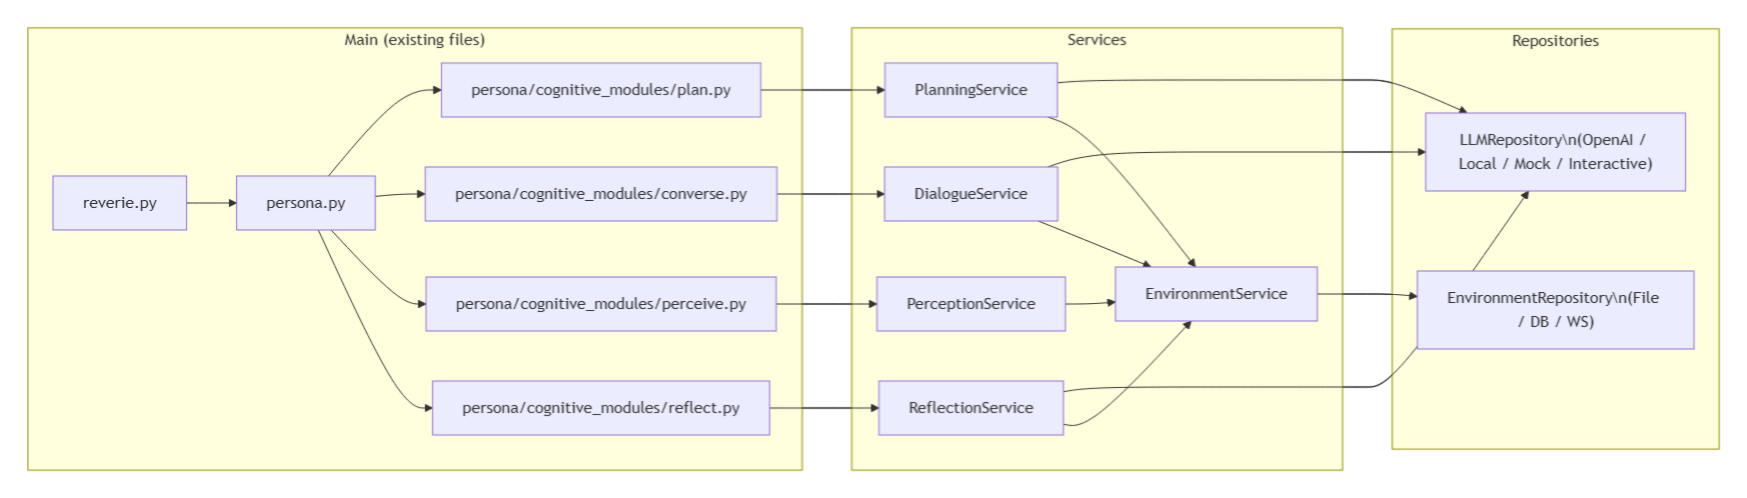
\includegraphics[width=\textwidth]{Pictures/Code Structure - after.png}
  \caption{Refactored service-oriented architecture with Repository, Service, and Orchestration layers. The \texttt{PlanningService} abstraction enables controlled comparison between baseline and neuro-symbolic planning implementations.}
  \label{fig:code-structure-architecture-after}
\end{figure}

\subsection{Prompt Templates}
All calls to the LLM are formalized using prompt templates that specify the system prompt [Maybe add what is that], few-shot examples, and templates for the actual prompt and expected output using OpenAI structured output, which allows us to constrain the model output. This also provides clear versioning of prompt templates.

\subsection{Model Used}
Most testing was conducted with the OpenAI model gpt-5-nano-2025-08-07, due to: 1. Cost-effectiveness, which is important considering our expected token usage to generate one simulation was 1m+; 2. Speed; 3. Reasoning capabilities with good benchmarks; 4. The ability to trade off "intelligence" versus speed by setting the reasoning token budget (reasoning effort between low, medium, and high).

  [Should we write about other models as well? like wht didn't we use mini normal gpt-5  - becouse of the price]

We also tested opensource models Qwen3:7b and gpt-oss:20b using Ollama as LLM engine on DGX spark [it's easy to setup and support structured output] The quality was similar to gpt5 nano but the infrence speed what about 10 time slower which stoped us from exploring this posobilities futher

\subsection{Long-Term Planning}
\label{Long-term planning}
As part of the improvements to the original architecture, we modified the prompts responsible for planning, as well as the surrounding code.
\subsubsection{Movement}
The biggest change is the programmatic addition of movement actions. In the original paper, characters moved as part of determined actions; for example, if an agent planned to eat breakfast for 20 minutes in a coffee shop that is 25 minutes from their current location, they would walk to the café for 20 minutes and, without even reaching the café, would start another activity. In our opinion, this reduced the believability of the original approach, so we decided to automatically block time for the movement activity. This ensures that the agent always has time to reach the destination before starting actions. However, it also requires estimating the time the agent will spend moving for each task during planning, as the action location is determined only after decomposing the task into actions.


\subsubsection{Daily Planning}

In the original paper, each task, such as "morning routine," was always generated as a multiple of one hour. With newer models and enforced structured output, we were able to ask the model to generate arbitrarily long tasks for a day. Another improvement is asking the model to generate task intent, what type of actions we expect to be necessary and the location of interest for the task---the area where the agent will most likely move during task execution.
We use task intent as context for prompts that will operate on the task [replanning, task decomposition]. Locations of interest are used to estimate travel time during the activity.

\subsubsection{Task Decomposition}
When an agent approaches a task that has not yet been decomposed, we trigger the task's decomposition into atomic actions. In the original implementation, each action was a multiple of 5 minutes, which produced some unbelievable actions, such as washing hands for 5 minutes. In our implementation, we allow the model to arbitrarily choose the duration in minutes. If neuro-symbolic validation is enabled, we enter the validation loop. Then, with the final task decomposition, we ask the model for the most appropriate place to perform each action. We then programmatically generate movement actions if the agent needs to switch locations between actions. Finally, we check if the total time is above or below the expected time for the task. We define the difference as delta [the time for the task itself vs. the expected time for the movement]. If we need to fill time, we add a "Checking phone" activity for |delta| minutes. If delta > 0, we need to decrease the time spent on actions. We achieve this by randomly decreasing the duration of activities by one minute, weighting activities that take longer so that a 20-minute activity has a ten times higher chance of being selected for decrease than a 2-minute activity [make the examples more mathematically strict].



\subsection{Neuro-Symbolic Validation Pipeline}
\label{subsec:neuro-symbolic-pipeline}
We implemented the following neuro-symbolic validation pipeline to enhance the coherence of actions generated during task decomposition. This is performed after generating actions from the task, but before adding movements.

\begin{figure}[H]
  \centering
  \includegraphics[width=\textwidth]{Pictures/methodology/NS_pipeline.png}
  \caption{Neuro-Symbolic Pipeline. Blocks with red outlines indicate LLM calls.}
  \label{fig:ns-pipeline}
\end{figure}

[TODO add example] We check the validity of preconditions using the external symbolic validation tool, VAL\cite{howey2004val}. To receive feedback from VAL, we must generate three files: Domain.pddl, Problem.pddl, and plan.pddl. Below, we explain how we achieved this.

\subsubsection{Domain Generation}
Domain generation is the most challenging part of the process [Because it's the biggest mental load, maybe add statistics for this. I mean it's just that the domain needs the most attention and problems here will propagate to following steps of the pipeline], and we tested a couple of approaches to do it correctly. The steps below generated the best Domain, based on our subjective assessment [We tested a lot and looked which generated more sensible results and which generated fewer validation errors]. We initially attempted to generate the entire PDDL file in one step, but encountered two problems: 1. Action conditions and effects tended to be chained without real logic. [add example, like teeth-brushed as precondition of shower]. After many iterations, we decided to split domain generation into the following steps.

  [Also we use structured JSON output to ensure proper naming and structure, and we should write about it we also tested temporal domain, but decided to focus on non-temporal one becouse it reduced the output token by [x] percent and was simple for model to generate]

\paragraph{Natural Language Precondition and Effect Generation}
We ask the model for natural language conditions and effects for each action separately to prevent the chained condition-effect problem.
\begin{verbatim}
Action: completing morning routine (Eat toast with fruit and drink coffee)
Preconditions:
  - Isabella is at home in the kitchen.
  - Bread for toast is available.
  - Fruit is available for breakfast.
  - Coffee is available and a means to drink it (cup/mug) is available.
  - A means to prepare toast (toaster or similar) is available.
Effects:
  - Toast is prepared and eaten (toast consumed).
  - Fruit is eaten (fruit consumed).
  - Coffee is drunk (coffee consumed).
  - Isabella's breakfast is completed/consumed.
\end{verbatim}

\paragraph{Predicates Generation}
We gather all natural language conditions and effects for each action, along with the world description, and ask the model to create a sensible predicate catalog with a focus on logical coherence. We do this in one step to ensure a unified set of predicates. As the domain is unique for a specific agent and specific task decomposition, we ask the model to generate zero-arity predicates, as we observed that this decreases hallucinations and malformed output from LLMs in subsequent stages of the pipeline.
\begin{verbatim}
- in_apartment: Is Isabella located inside her apartment.
- lying_down: Is Isabella lying down in bed.
- coffee_available: Coffee (grounds or beans) is available to brew.
- bread_available: Bread is available to toast.
- toaster_functional: Toaster is functional for toasting bread.
- toast_toasted: Toast has been toasted and is ready to eat.
- breakfast_completed: Breakfast is completed.
...
\end{verbatim}


\paragraph{PDDL Action Schema Generation}
Now, for each action, we generate an action schema from the predicate catalog and natural language conditions and effects. We do this separately for each action to avoid encouraging condition and effect chaining. Afterward, we programmatically create the domain file.
\begin{verbatim}
(:action eat_toast_with_fruit_and_drink_coffee
    :parameters ()
    :precondition (and
      (bread_available)
      (toaster_functional)
      (toast_toasted)
      (fruit_available)
      (coffee_available)
      (cup_available)
      (coffee_maker_functional)
    )
    :effect (and
      (toast_consumed)
      (fruit_consumed)
      (coffee_consumed)
      (breakfast_completed)
      (cup_empty)
      (not (bread_available))
      (not (toast_toasted))
      (not (coffee_available))
      (not (fruit_available))
    )
)
\end{verbatim}

\paragraph{Validation with VAL and Repair}
We check domain validation using the VAL tool. The main purpose is to ensure the model did not hallucinate new predicates or create malformed PDDL schemas.
If there is an error, we pass the feedback to the LLM to generate the repaired domain. For instance, if VAL reports \texttt{Use of undeclared predicate: (feeling\_good)}, the LLM will add \texttt{(feeling\_good)} to the predicates list and regenerate the domain.

\subsubsection{Problem Generation}
After successfully generating the domain, we ask the LLM to generate the problem based on the predicate catalog, the current state of the world, and the task intent. From this, we obtain the initial state of the world and the goal. After generation, the domain and problem files are fed to VAL to check for syntax problems and potential hallucinations; the problem is regenerated with VAL feedback in case of errors.
\begin{verbatim}
(define (problem isabella_morning_routine)
  (:domain persona_world)
  (:init
    (in_apartment) (lying_down) (bed_area_clear)
    (water_running_in_sink) (sink_functional)
    (toothbrush_available) ...
  )
  (:goal (and
    (breakfast_completed)
    (toast_toasted)
    (cup_available)
  ))
)
\end{verbatim}

\subsubsection{Plan Generation Programmatic}
As we use zero-arity predicates, the actions also become zero-arity, allowing us to automatically generate the problem file from the original decomposed actions.
\begin{verbatim}
0: (sit_up_in_bed_and_stretch) 
1: (put_on_robe_and_adjust_pillows) 
2: (wash_face_brush_teeth_and_apply_skincare) 
3: (brew_coffee_and_toast_bread) 
4: (eat_toast_with_fruit_and_drink_coffee) 
\end{verbatim}

\subsubsection{VAL Analysis}
We input the domain, problem, and plan files into VAL and continue based on its feedback.
\begin{verbatim}
Checking next happening (time 4)
Plan failed because of unsatisfied precondition in:
(eat_toast_with_fruit_and_drink_coffee)
Deleting (bread_available)
...
Goal not satisfied

Plan Repair Advice:
(eat_toast_with_fruit_and_drink_coffee) has an unsatisfied 
precondition at time 4
(Follow each of:
    (Set (bread_available) to true)
    and (Set (fruit_available) to true)
    and (Set (coffee_available) to true)
)
\end{verbatim}
If the plan is valid, we end the pipeline. If there are any errors, we move to the next step in the validation pipeline.

\subsubsection{LLM Feedback}
If VAL reports an error, we input the context of the generated PDDL artifacts and feedback from VAL, then ask the LLM to generate actionable responses for each error found. The model can choose between:
\begin{itemize}
  \item \texttt{ok} - can continue (when the error is due to an incomplete problem init state [Example: no phone in the world state])
  \item \texttt{pddl\_error} - There is an error in PDDL itself
  \item \texttt{need\_replan}
\end{itemize}
Based on all error items, the model decides on one of three actions:
\begin{itemize}
  \item \texttt{ok} - we end the pipeline and assume the plan is valid
  \item \texttt{pddl\_repair\_required} - we repair each of the PDDL artifacts with feedback from VAL and then perform VAL evaluation again
  \item \texttt{replan\_required} - we continue with the pipeline
\end{itemize}
\begin{verbatim}
{
  "feedback_items": [
    {
      "error_description": "Final action 'Eat toast...' cannot be executed 
      because its preconditions are not satisfied: bread_available, 
      fruit_available, and coffee_available are not true...",
      "category": "need_replan",
      "recommendation": "Replan to remove the final eating step..."
    }
  ],
  "overall_next_action": "replan_required"
}
\end{verbatim}

\subsubsection{Replan Goal}
This stage creates a natural language replanning goal based on the feedback from validation and the current schedule, as well as task intent. We added this stage as we noticed that feeding PDDL feedback to the replanner generates poor results.
\begin{verbatim}
Insert 'Restock bread, fruit, and coffee' before 'Eat toast with 
fruit and drink coffee'
\end{verbatim}
\subsubsection{Replanning}
In this stage, we ask the LLM to generate a new plan based on the replanning goal and the current schedule.

We repeat the pipeline above a set number of times.


\section{NL Condition Validation}
\label{subsec:NL-conditions-validations}
After the validation pipeline, we store the natural language preconditions for each action. When the action begins, we check if the preconditions still hold; if not, we replan.
\subsection{Checking NL Condition}
At the beginning of each action (when the agent is about to execute the action), we retrieve the state of objects in the world around the agent, as well as other memories relevant to the conditions, for each condition. We then ask the model to categorize the condition as satisfied or not, based on this information and common sense.
\begin{verbatim}
Action: Head to Hobbs Cafe and open for the day (Greet the first 
guests as they arrive)
Condition: At least one guest has arrived at the cafe entrance.
Result: {
  "is_satisfied": false,
  "probability": 0.35,
  "reasoning": "As of 08:00 on Feb 13, 2023, World State shows the cafe 
  behind the counter idle with no indication of guests at the entrance. 
  Therefore, condition 'at least one guest has arrived' is not satisfied."
}
\end{verbatim}
If all conditions are satisfied, the agent will start the action.
\subsection{Replan Goal}
If at least one condition is not satisfied, we ask the LLM to generate a replanning goal based on the schedule, the agent's daily goal, and the violated conditions.
\begin{verbatim}
Action: Head to Hobbs Cafe and open for the day (Greet the first 
guests as they arrive)
Failed Conditions: [
  {
    "condition": "At least one guest has arrived at the cafe entrance.",
    "reasoning": "As of 08:00... no indication of guests..."
  }
]
Result: {
  "modification_goal": "Replace 'Greet the first guests as they arrive' 
  with 'Wait for the first guest at Hobbs Cafe entrance'",
  "reasoning": "The condition ... is not satisfied ... corrective 
  action is to wait..."
}
\end{verbatim}
\subsection{Replan Next 2h}
We then ask the LLM to replan the next 2 hours with the replanning goal in mind. [example]



\section{Quantitative Evaluation: Constraint Violation Analysis}
\label{sec:quantitative-evaluation}

[To be completed: automated evaluation comparing the hierarchical planning baseline against our validator-augmented system. The validator will automatically detect and flag constraint violations such as attempting to use items that are not available, scheduling overlapping activities, violating location constraints, or executing actions whose preconditions are not satisfied. Metrics will include violation counts at day-level and action-level, violation rates per 100 actions, and success rates after optional validator-guided repair rounds.]



\section{Experimental Setup}
\label{sec:experimental-setup}
For the user study, we generated two simulations: baseline and neuro-symbolic. Since the focus of our study was how neuro-symbolic planning can increase the believability of LLM-based agents, we decided to isolate as many variables as possible.
Both simulations featured the same three personas with backgrounds taken from the original study. We generated exactly the same goals and tasks for the day [for each persona] for both simulations.
Both the baseline and neuro-symbolic models used the improvements introduced in \ref{Long-term planning}.
Thus, the generation differed only by the introduction of validations in the neuro-symbolic simulation \ref{subsec:NL-conditions-validations} \ref{subsec:neuro-symbolic-pipeline}.

We tested generating simulations of a world with 25 characters, but the improvements in believability [our subjective assessment] did not justify the additional cost in tokens and the increased effort required for test subjects to complete the study.

For both simulations, we implemented extensive logging to understand system behavior. We log:
\begin{itemize}
  \item Usage of each generation template, including the number of calls and tokens spent.
  \item Every broken validation with context [The PDDL files or NL condition that was broken].
  \item Every replanning goal.
  \item Every modification to the plan time [when the movement takes too much time].
\end{itemize}


\section{User Study: Believability Evaluation}
\label{sec:user-study-believability}

This section describes the human-subjects study testing whether a simulation generated with the neuro-symbolic validation approach improves perceived believability of agent behavior compared to the our baseline reimplementation of Generative Agents architecture \cite{parkGenerativeAgentsInteractive2023a}. We focus on the believability of \emph{actions} rather than solely on personalities or conversations.

\subsection{Objectives and Hypotheses}
\label{subsec:objectives-hypotheses}

Two primary hypotheses:

\begin{itemize}
  \item \textbf{H1 (overall believability)}: Participants judge agents powered by our method as more believable overall than the baseline in matched scenarios.
  \item \textbf{H2 (action believability)}: For the same scenario, participants flag fewer actions as ``unbelievable'' in our method than in the baseline.
\end{itemize}

Secondary outcomes: (i) free-text reasons participants provide when deeming actions unbelievable (used for qualitative error analysis) \cite{batesRoleEmotionBelievable1994,bogdanovychWhatMakesVirtual2016,tenceAutomatableEvaluationMethod2010,xiaoHowFarAre2024}.

\subsection{Conditions}
\label{subsec:conditions}

Two within-subject conditions on the same simulated world and character seeds:

\begin{enumerate}
  \item \textbf{Baseline (GA)}: Improved re-implementation of Generative Agents \cite{parkGenerativeAgentsInteractive2023a}.
  \item \textbf{Ours (Neuro-symbolic)}: Proposed system with symbolic planning and consistency checks integrated into deliberation and action selection.
\end{enumerate}

Each participant evaluates both conditions on the same character and scenario to enable within-subject comparison. Order is counterbalanced to reduce presentation effects.

\subsection{Participants}
\label{subsec:participants}

We targeted 10 to 15 adult participants recruited from the university community and online platforms. Inclusion criteria: English proficiency. We conducted an initial pilot (3 to 4 participants) to validate timing and interface, then proceeded to the main study. All participants provide informed consent and can withdraw anytime without penalty.

Due to recruitment constraints, our participant pool is limited, which precludes a rigorous ablation study\footnote{An ablation study systematically removes or disables individual components of a system to measure their independent contributions to overall performance.} isolating the contribution of individual components (e.g., symbolic validation versus NL condition checking). This approach mirrors that of the original Generative Agents work \cite{parkGenerativeAgentsInteractive2023a}, which also evaluated the system holistically through user studies. Instead, we evaluate the neuro-symbolic system as an integrated whole through the believability study and constraint violation analysis described in Sections \ref{sec:quantitative-evaluation} and \ref{sec:user-study-believability}.

\subsection{Materials and Stimuli}
\label{subsec:materials-stimuli}

The stimulus for each condition is a replay of a single random character's day. To focus on action believability, we present:

\begin{itemize}
  \item time-lapse \emph{video replay} of the agent acting in the world (controllable playback speed, pause/seek);
  \item Activity log with details about the current activity and animated time tracking; and
  \item UI controls to mark an action as unbelievable (``thumbs down''), provide a short reason, and continue.
\end{itemize}

Replays cover the same scenario (e.g., two simulated in-game days) and use the same character profile, task for the day and randomness seed across conditions, so any variation is attributable to agent architecture (baseline vs. ours) rather than scenario noise.

\subsection{Procedure}
\label{subsec:procedure}

Each session (approximately 30 minutes):
The user reads the paper version of the user guide, while the evaluator follows the evaluator guide.
\begin{enumerate}
  \item \textbf{Introduction.} A scripted briefing introduces the task and believability as coherence, plausibility, and consistency within world rules \cite{bogdanovychWhatMakesVirtual2016}.
  \item \textbf{Practice.} Participants complete a 2 to 3 minute tutorial on the interface using a neutral example not used in the main study.
  \item \textbf{Condition A.} Watch the replay, freely scrub, and mark unbelievable actions. For each mark, add a short explanation (optional but encouraged).
  \item \textbf{Condition B.} Repeat with the other planner. Order varies across participants; assignment is double-blind.
  \item \textbf{Summary.} We show the user an overview of marked actions in both conditions and ask which one felt more human-like.
\end{enumerate}

We record and transcribe the experiment for a later qualitative study of unbelievable actions.
The experiment was conducted using a custom-developed website (Figure \ref{fig:study-interface}).

\begin{figure}[H]
  \centering
  \includegraphics[width=\textwidth]{Pictures/methodology/Study_interface.png}
  \caption{User interface for the study, showing the replay view and mechanism for flagging unbelievable actions.}
  \label{fig:study-interface}
\end{figure}

\subsection{Measures}
\label{subsec:measures}

[Do we need to write anything here?]

\subsection{Data Quality and Exclusion}
\label{subsec:data-quality}

Sessions are excluded if participants fail an attention check (simple comprehension question about the replay), leave more than half the session unanswered, or complete in less than one-third of median time. We pre-register exclusion rules prior to data collection.

